\documentclass[a4paper, 12pt]{article}
\usepackage[utf8]{inputenc}

\usepackage{amsmath}
\usepackage{graphicx}
\usepackage[top=1in, bottom=1in, left=1in, right=1in, textheight=24cm]{geometry}
\usepackage{float}
\usepackage{enumitem}
\usepackage{url}
\usepackage{natbib}
\setlength{\parindent}{0pt}

\title{Image Classification Project Report}
\author{Gradient Descendants: \\Cardin Christian, Nieminen Harri, Zetterman Elina}
\date{\today}

\begin{document}

\maketitle

\section{Introduction}
Image classification is a fundamental problem in computer vision that involves assigning a single label to an image that best describes its contents. Traditional image classification tasks are typically single-label, meaning that each image is assigned to a single category. However, in many real-world applications, images may belong to multiple categories simultaneously. This is known as multilabel image classification, and it presents unique challenges compared to single-label classification.


In this project, we focus on developing a deep learning model for multilabel image classification. We use the provided dataset, which consists of 20000 images labeled with 14 possible categories: ['baby', 'bird', 'car', 'clouds', 'dog', 'female', 'flower', 'male', 'night', 'people', 'portrait', 'river', 'sea', 'tree']. The goal of this project is to achieve high accuracy on this dataset and demonstrate the potential of deep learning for multilabel image classification.

\subsection{Data Analysis}
\begin{figure}[h]
    \centering	
      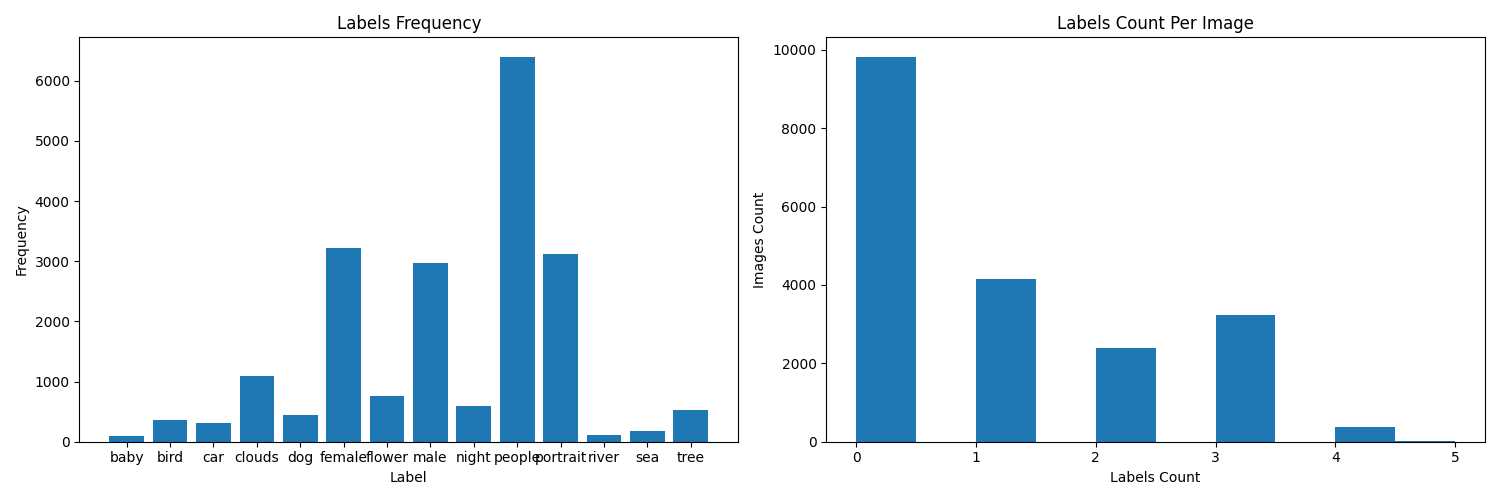
\includegraphics[width=0.95\textwidth]{"img/labels.png"}
    \caption{Visualization of labels frequency}
    \label{fig:labels}
\end{figure}


%\begin{itemize}
%\item Total images: 20000, Unlabeled images: 9824, Labeled images: 10176, Ratio: 0.5088
%\item Each image is 128x128 pixels in size.
%\item Mention that the dataset is unbalanced, with some categories having many more images than others, and the majority is unlabeled.
%\item We did not do any preprocessing of the images, but in the code we do a normalization of the pixel values and we have the option to load the image as grayscale.
%\item Data augmentation: did we try anything?
%\end{itemize}

The data set we were given contains a total of 20000 images, 9824 of which are completely unlabeled, and 10176 of which had one to five labels, as seen in the right hand side plot of figure~\ref{fig:labels}. As the left hand side plot of figure \ref{fig:labels} shows, the data set is quite unbalanced, with some categories having noticably more images than others.


The data set contains both black-and-white and colored images, and each image is 128x128 pixels in size. For the final model, we have not done any preprocessing of the images, but we have normalized the pixel values of the images. When training the model, we experimented with multiple data augmentation options including image resizing, rotations and cropping, image level alterations and random erasing. However as the results of data augmentation varied greatly on different  proportions of the imageset at hand, the approaches tried were deemed too unconfident to be utilized for the training of the final model. The only prevailing image alteration for the training is the option to load in all images as either grayscale or rgb, which allows us to compare how including the color impacts the accuracy of the model.



\section{Methods}

\subsection{Software Architecture}

%\begin{figure}[h]
%	\centering	
%	  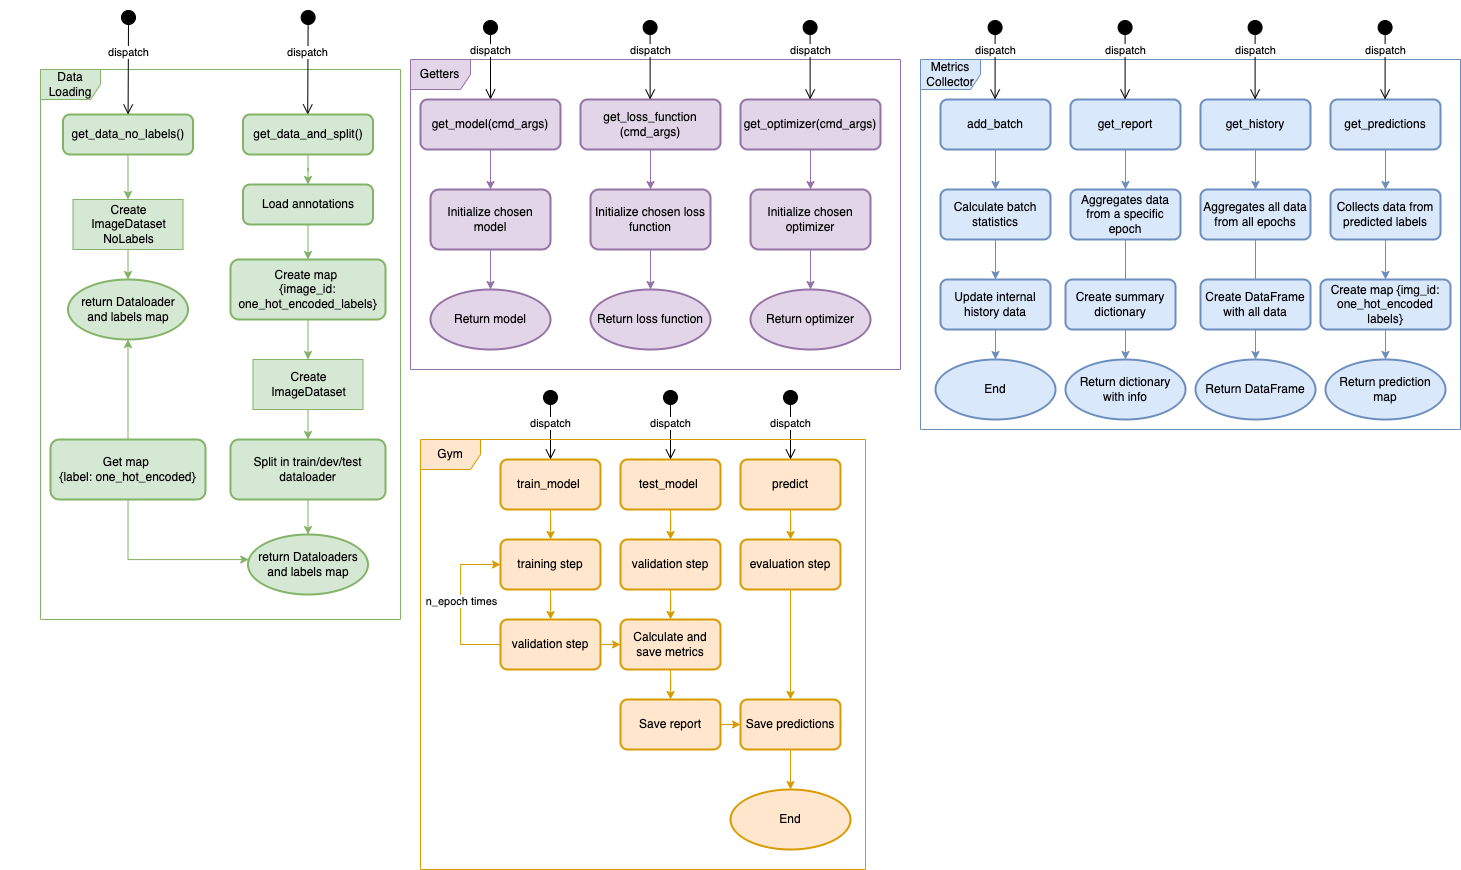
\includegraphics[width=0.95\textwidth]{"img/arch.png"}
%	\caption{Abstraction of the software architecture.}
%	\label{fig:arch}
%\end{figure}

The architecture can be summarized in for main parts: Data loading, model and parameter selection, model training and metrics collection.

\paragraph{Data Loading:} 
Our system's data loading process is crucial for preparing input data for model training. It involves reading command line arguments for setting loading and training parameters such as hyperparameters (e.g., epochs, learning rate, image color mode, loss function, optimizer, batch size) and model selection. Debug options such as verbosity level, dataset size, and pre-trained model loading are available to enable flexible experimentation and facilitate easy training process fine-tuning.

We load annotation files to create a mapping between each image ID and its corresponding collection of one-hot-encoded labels. For example, an image with ID 12345 might have labels [0, 1, 1, 0, 0, 1, ...], where each value corresponds to a category (e.g., 'baby', 'bird') and indicates whether the image belongs to that category (1) or not (0).

Image loading occurs in a custom \texttt{ImageDataset} class that returns a combined tuple of \texttt{[image\_data, labels, image\_ids]} to keep track of training, validation, and test history. The \texttt{ImageDataset} applies transformations such as normalization and setting the color mode, and caching options for faster training. The dataset is split into train, validation, and test DataLoaders, with batch size specified based on the input command arguments.

\paragraph{Gym (training and evaluation):} 
The \texttt{Gym} class is responsible for training and evaluating the model. To begin with, the class is initialized with a set of hyperparameters, a chosen loss function, an optimizer, and the target model. During the training phase, the \texttt{Gym} trains the model for a specified number of epochs, recording the loss and accuracy for each iteration. Furthermore, the \texttt{Gym} keeps track of the training history thanks to the \texttt{MetricsCollector} helper class, allowing for the easy plotting of accuracy and loss curves. In "test mode", the \texttt{Gym} uses the \texttt{MetricsCollector} class to collect all predictions and subsequently calculate useful metrics like the F1 score and confusion matrix for the entire dataset. Additionally, the \texttt{Gym} offers the option to load a pre-trained model for evaluation purposes only.

\paragraph{Metrics Collector:} 
It is responsible for calculating and storing per-batch statistics during model training, which are later aggregated to create per-epoch statistics. Additionally, the MetricsCollector saves the model's predictions alongside the ground truth at each iteration. This enables us to generate useful metrics such as accuracy scores, F1 scores, and confusion matrices, which are used to compare the performance of different models. Thanks to the MetricsCollector, we can evaluate the effectiveness of our models and fine-tune our training process accordingly.

\paragraph{Getters:}
A very simple module that inspects the command line arguments to return the correct objects for the model, loss function, and optimizer. This allows us to easily switch between different components without having to manually change the code between experiments.

\subsection{Models Architecture}
%[TODO]: Should we put something about the performances of the models here? No, we can compare the performances in the results

We implemented a few different models and tried them with different accuracy metrics and loss functions. A total of six models were implemented (including a dummy model), a couple of which are described more in detail below.

The first model implemented consists of four convolutional layers, each with relu activation and maximum pooling, and two linear dropout layers, each with relu activation. The output layer is a linear layer with sigmoid activation.

Another model we tried has three convolutional layers, each with batch normalization, relu activation, and maximum pooling. The model also has one linear layer with relu activation, and a linear output layer with sigmoid activation.

The final model that we implemented has five convolutional layers, each with relu activation, batch normalization, and average pooling. The first, third, and fifth layers also use the dropout method. After the convolutional layer is a linear layer with relu activation, batch normalization and dropout. The output layer is a linear layer with sigmoid activation.

\subsection{Training and Evaluation}
%[TODO]

%\begin{itemize}
    %\item Describe the training process
    %\begin{itemize}
    %    \item How did we split the data?
    %    \item What metrics did we use (accuracy/loss/f1) and how did they calculate them (mention the threshold used for determining correctness)?
    %    \item How did we choose the hyperparameters?
    %\end{itemize}
    %\item Describe the evaluation process
    %\begin{itemize}
    %    \item how do we compare different models to see which one is better?
    %\end{itemize}
    %\item List the regularization and optimization techniques we used (Data normalization, data augmentation, dropout... any more?). We did not use early stopping, but at least I haven't seen any opportunity where we could have benefitted from it, looking at the accuracy plots.
    %\item Are there other things that we considered, but did not have time to implement?

%\end{itemize}

First, the data is split randomly into training, validation, and testing sets. For training the final model, the data was only split randomly into training and validation sets, since we are given a new testing data set for which to make predictions. The fraction of data to use for training can be specified as a parameter, and by default, the data is split 80--10--10 for training, validation, and testing, respectively. For the final model, 85~\% of the data was used for training, and the rest for validation. % change depending on final model

The optimizer and loss function can also be given as a parameter. The list of optimizers includes AdamW, Adam, stochastic gradient descent (SGD), Adamax, and Adadelta. The list of loss functions includes binary cross entropy loss (BCE loss), multilabel softmargin loss, mean squared error loss (MSE loss), and L1 loss. The final model was trained using BCE loss and Adadelta.  % change depending on final model

Most of the hyperparameters (batch size, learning rate, number of epochs, etc.) can be specified as command line arguments. The final hyperparameters were chosen mostly through trial and error, by comparing how different values impact the accuracy, f1 score and confusion matrix. % CONFIRM THIS
For the final model, the hyperparameters used were a batch size of 32, a learning rate of 0.2, and 15 epochs. % change depending on final model
Another important hyperparameter is the threshold for prediction, which gives the minimum probability the model has to assign to a label in order for the model to predict that label to belong to the image.

The main metric used for comparing the different models is validation accuracy and confusion matrix on the test dataset. Other metrics that are calculated are micro and macro precision, recall and f1-score over the training and validation phases. The scores calculation is done in the \texttt{MetricsCollector} class (check source code for more details).

On top of these, validation accuracies of each individual label are also calculated. Different models are compared by looking at plots of these accuracies, as well as training/validation loss, as a function of the epoch.

Regularization/optimization techniques used include within-batch data normalization and the dropout method. Early stopping was also considered, but seeing that the validation loss remained around the same value for all epochs, we decided that it might not help improve the model significantly. Another method that was considered is data augmentation, but unfortunately, we did not have time to fully implement this. % if data augmentation was tried, add here how it went

Moreover, our software supports different modes of operation:
\begin{description}
  \item[\textbf{train}] Creates an empty model, trains and evaluates it on the provided train data. The output gives a full report on the performance and the trained model's weights.
  \item[\textbf{eval}] Loads a model from a weights file, evaluates it on the provided labelled test data, reporting its performance.
  \item[\textbf{pred}] Loads a model from a weights file, evaluates it on the provided unlabelled test data, and outputs a .tsv prediction file. 
\end{description}

To learn more about how to run the code, refer to the README.md in the project's folder.

\section{Results}
%[TODO] 
%\begin{itemize}
%\item Show accuracy plot and confusion matrix for the best model. 
%\item Perhaps have a discussion about the difference between training with and without unlabeled data. 
%\item Are the result good? What is our interpretation and opinion?
%\item Do we have any expectation on the model's real accuracy?
%\item Self-reflection: What could we have done better? What can we still do? % data augmentation, if we did not try it
%\end{itemize}

The model used to make the final predictions is the ResNet50 model from Pytorch \cite{pytorch}, which uses pre-trained weights. The model is trained on RGB versions of the images, with 85~\% of the data used for training, and 15~\% for validation. The loss function is BCE loss, and the optimizer is Adadelta. The batch size is 32, the learning rate is 0.2, the number of epochs is 15, and the threshold for prediction is 0.5.

The accuracies and evaluation metrics of the final model are shown in Figure \ref{fig:accuracy}. The micro precision is quite good, but the macro precision and overall validation accuracy have room for improvement. We would expect the accuracy of the testing set to be around the same range as the validation accuracy, so around 59\%. It's worth noting that the accuracy score is calculated considering a prediction "correct" only if all the picture's labels were predicted correctly. From the middle-left panel of Figure \ref{fig:accuracy} we see that the individual label accuracies are better than the "general" accuracy. The confusion matrices of different labels are shown in Figure \ref{fig:confusion_matrix}, calculated on the test set. It seems that the true positive are fairly decent, especially for categories that are more abundant like "people" and "portrait". On the opposite, "river" performed the worst, with 0 true positive predictions. We should have tried augmenting the data to eaven out the difference in frequency of the labels.

Our biggest concern about this model is that, according to the train/validation loss and accuracy, it seems to overfit the training data, and it's not able to generalize well. This can be especially noticed in the plots in the second row of Figure~\ref{fig:accuracy}, where it seems that validation metrics stay about constant throughout the epochs. However, even with this clear defect, this model still produced better predictions on the test dataset than every other model we tried, based on the confusion matrix and the aggregated micro and macro f1 scores (included in the final .zip package).

The model could be improved, for example, by trying different regularization methods, such as early stopping or data augmentation. We briefly tried data augmentation, but it did not seem to improve the accuracy. Therefore, if we had more time, we could experiment with different kinds of data augmentation. Another thing that could be done is research the subject and see what kinds of alternative model architectures are commonly used in other similar applications. Our software architecture is flexible and easily extensible to support different kinds of models quickly, with script to automate model testing, which was very useful in this project.



\begin{figure}[ht]
    \centering
    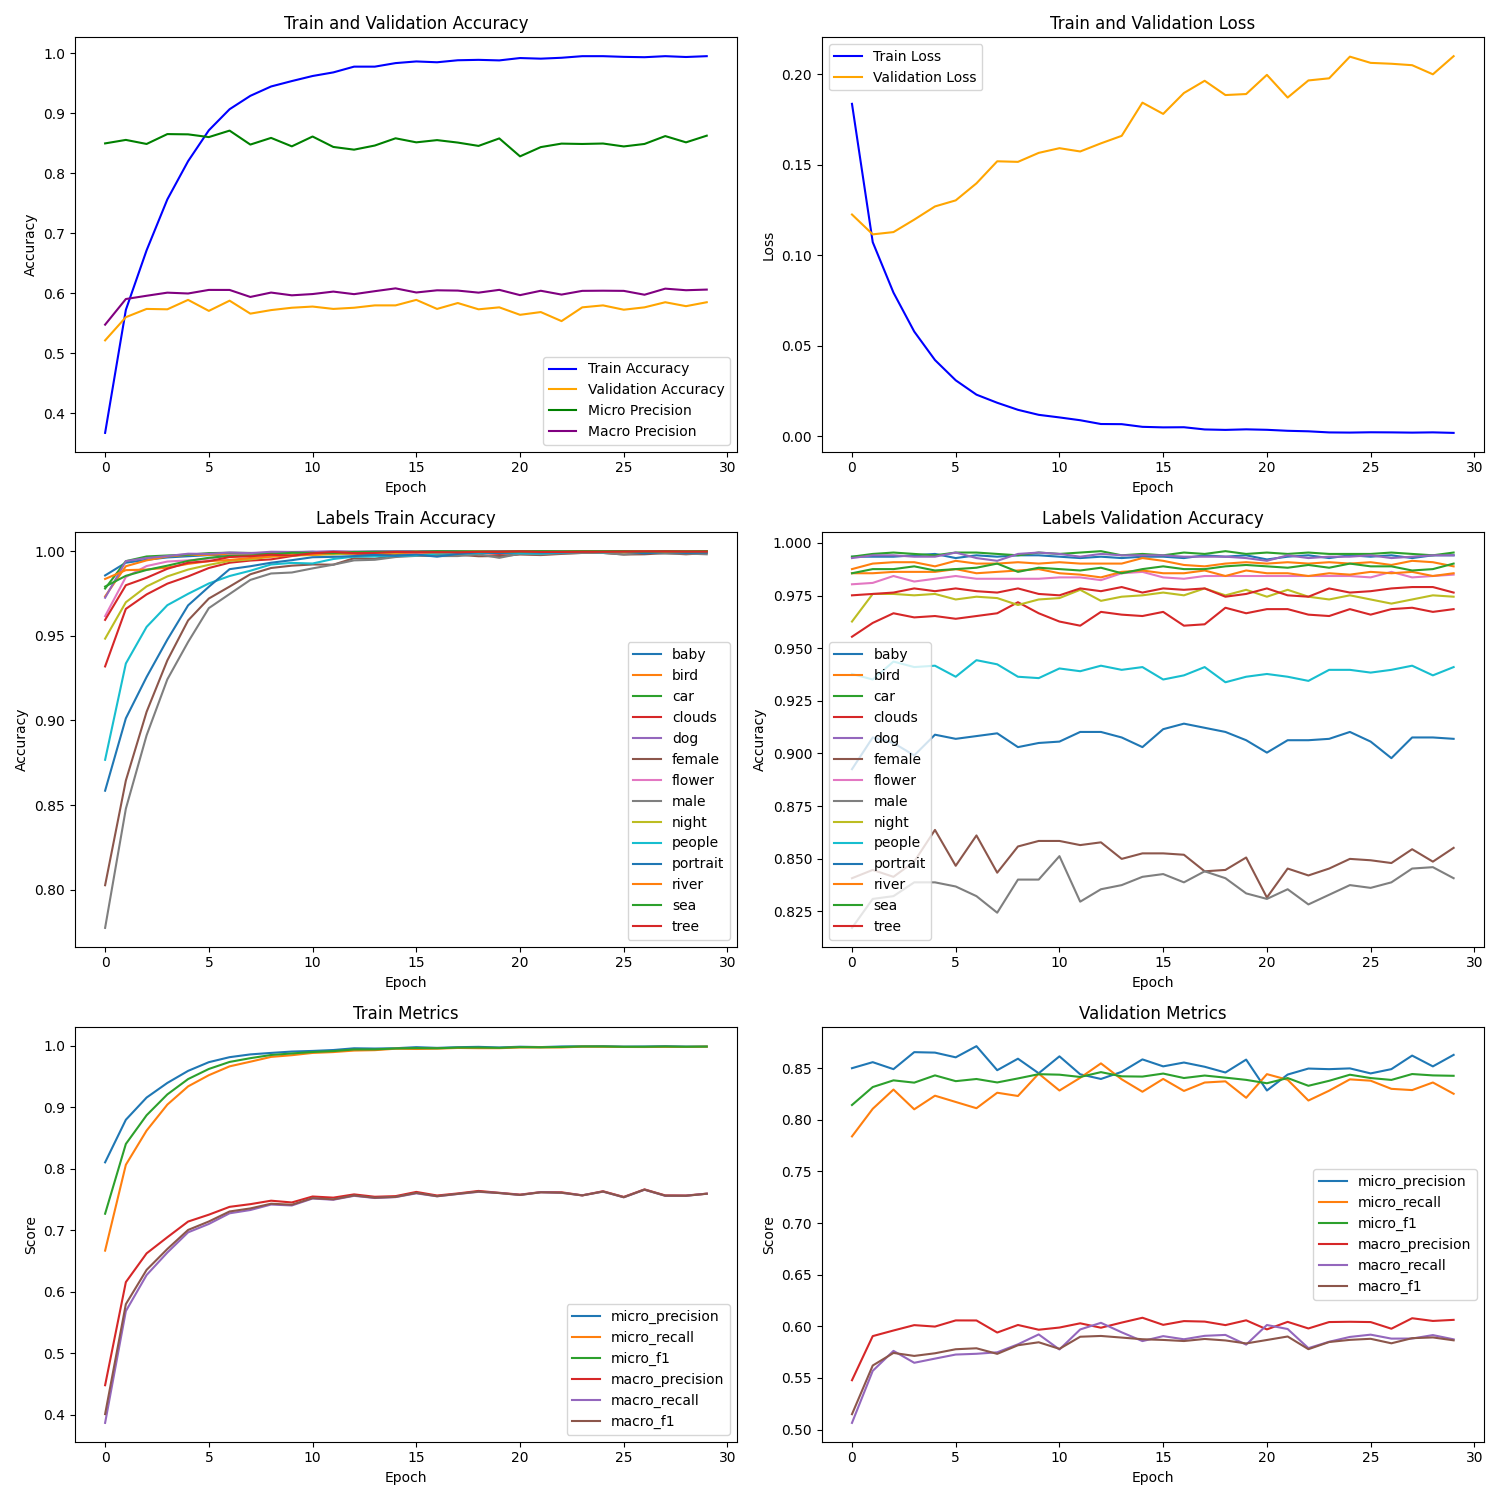
\includegraphics[width=\textwidth]{img/accuracy.png}
    \caption{Accuracies and evaluation metrics of the final model.}
    \label{fig:accuracy}
\end{figure}

\begin{figure}
    \centering
    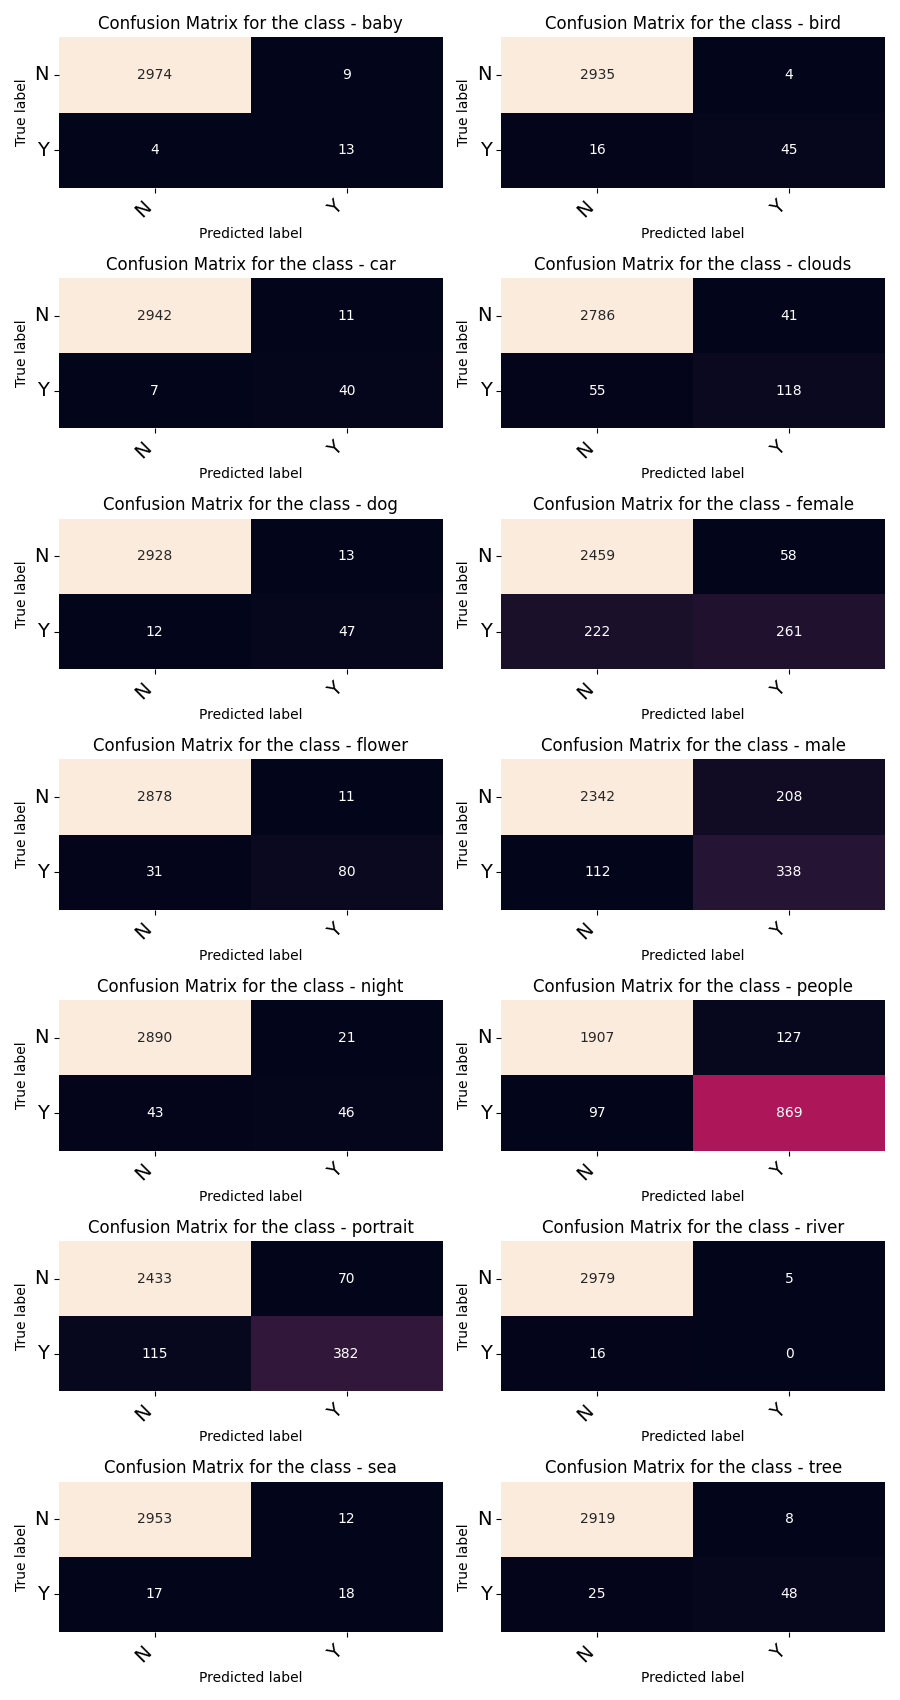
\includegraphics[width=0.7\textwidth]{img/confusion_matrix_test_dataset.png}
    \caption{Confusion matrices of the final model.}
    \label{fig:confusion_matrix}
\end{figure}

% add references
\renewcommand\bibname{References}
\bibliographystyle{abbrv}
\bibliography{references.bib}


\end{document}
